\documentclass[xcolor=table]{article}
\usepackage{graphicx}
\usepackage{ragged2e}
\usepackage{pstricks}
\usepackage{pst-eps}
\usepackage{pstricks-add}
\usepackage{anyfontsize}
\usepackage{pifont}
\usepackage{DejaVuSansMono}
\usepackage{libertine}
\begin{document}
\TeXtoEPS
\begin{pspicture}(0,0)(22,20)
%\rput[bl](0,0){\psgrid(0,0)(18,18)}
\rput[bl](1,0){%
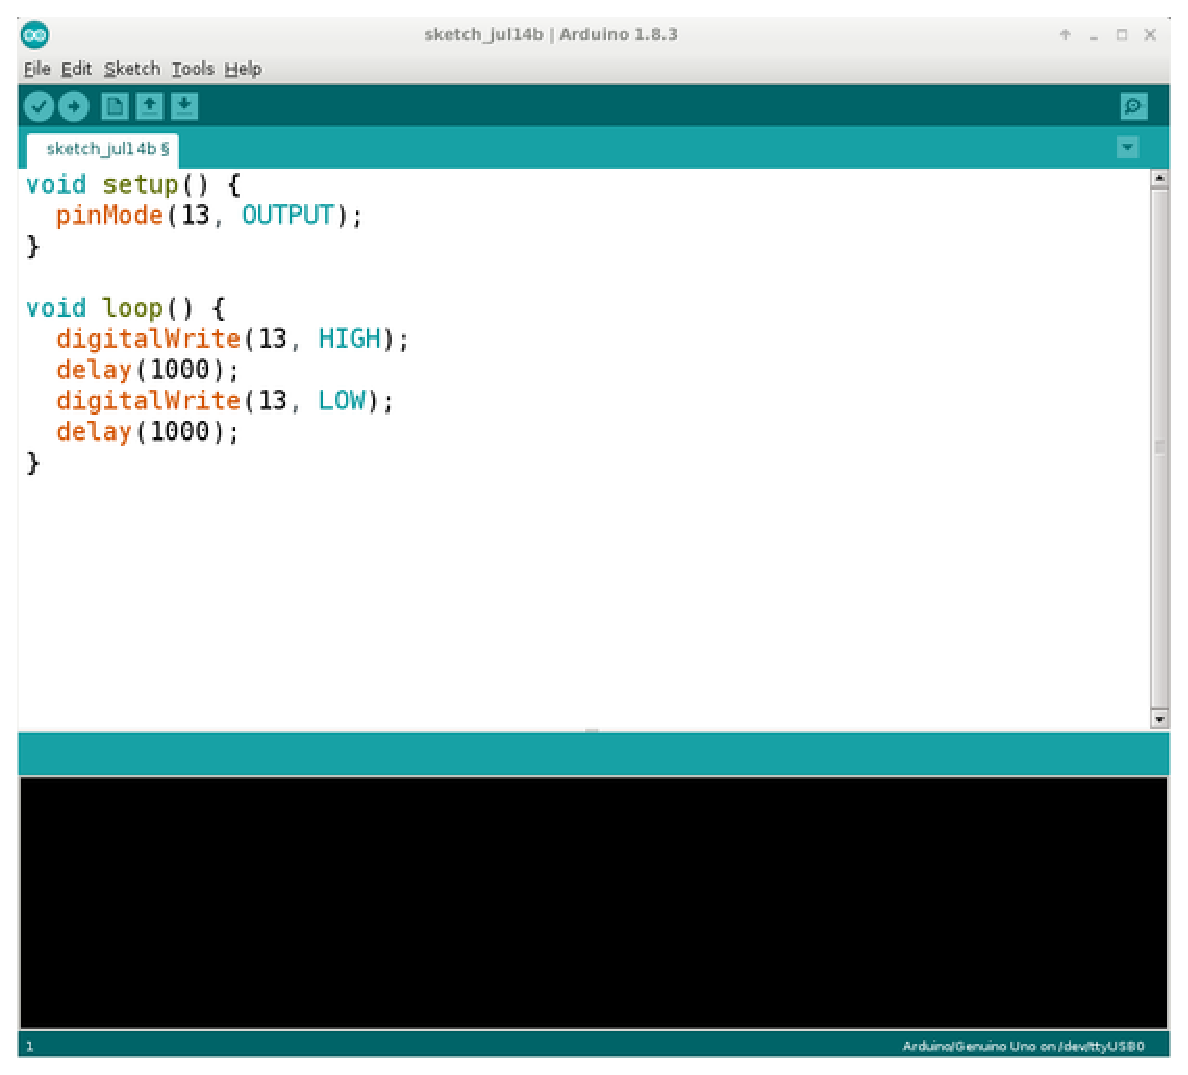
\includegraphics{screen.eps}
}
\psframe[linewidth=6pt,linecolor=red,framearc=0.12](0.85,5.5)(20.2,15.3)
\end{pspicture}
\endTeXtoEPS
\end{document}
